\documentclass[11pt]{book}
\usepackage{gvv-book}
\usepackage{gvv}
\usepackage[sectionbib,authoryear]{natbib}
\setcounter{secnumdepth}{3}
\setcounter{tocdepth}{2}
\makeindex
%
\begin{document}
\section*{NCERT 9.7.1.5}
\textbf{This Question is from ncert class 9  chapter 7.Triangles }
\begin{enumerate}
    \item Line $l$ is the bisector of an angle $\angle A$ and $B$ is any point on $l$. $BP$ and $BQ$ are perpendiculars from $B$ to the arms of $\angle A$. Show that:
%
\begin{enumerate}
    \item $\triangle  APB \cong \triangle AQB$  
    \item $BP$ = $BQ$ or $B$ is equidistant from the arms of $\angle A$.
 
\end{enumerate}
\end{enumerate}

\begin{figure}[H]
    \centering
    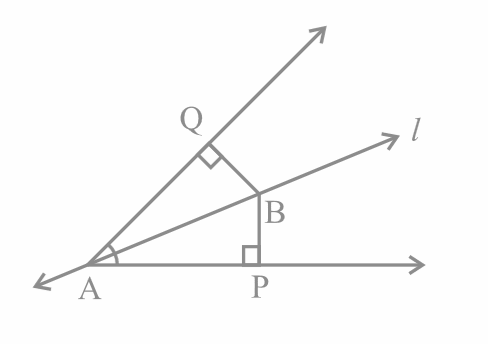
\includegraphics[width=\columnwidth]{fig_mc.png}
    \caption{$\triangle AQB \hspace{12pt} and \hspace{12pt} \triangle APB$}
   % \label{fig:math_comp1}
\end{figure}

\textbf{solution:}

Given $l$ is the angular bisector of $\angle QAP$ ,so $\angle QAB $ = $\angle PAB $ 
and $BP$,$BQ$ are perpendicular bisectors so angle =90$\degree$ .
%
let 
\begin{align}
	\angle QAB  = \angle PAB  =\theta = 30 \degree \\
	AP = r =4 \\
	AB = 5 \\
	\vec{A} = \myvec{0 \\ 0} ,\,
	\vec{B} = \myvec{5 \\ 0} ,\,
	\vec{P} = \myvec{r\cos(\theta) \\ -r\sin(\theta)} ,\,
	\vec{Q} = \myvec{r\cos(\theta) \\ r\sin(\theta)} \\
\end{align}

\begin{enumerate}
\item  
\begin{enumerate}
        \item By the definition of AAS (Angle Angle Side) congruency rule ,If two triangles have two equal angles and a pair of corresponding sides are equal then the two triangles said to be congruent.
%
Here
  \begin{align}
            \angle QAB  &= \angle PAB = 30\degree \hspace{12pt}   \text{($l$ is angular bisector of  $\angle QAP$)}  \\
            \angle AQB  &= \angle APB = 90 \degree  \hspace{12pt}  \text{($BP$ and $BQ$ are perpendicular bisectors)} \\
            AB &=5  \hspace{12pt}  \text{(common side for two triangles)} 
        \end{align} 
    $\therefore$ By AAS congruency rule  $\triangle  APB \cong \triangle AQB$  
    \item  \begin{align}
\norm{\vec{B}-\vec{Q}}\ &=  \sqrt{\brak{\vec{B}-\vec{Q}}^{\top}\brak{\vec{B}-\vec{Q}}} \\
\vec{B}-\vec{Q} &= \myvec{5 \\ 0} - \myvec{r\cos(\theta) \\ r\sin(\theta)} \\
\vec{B}-\vec{Q} &= \myvec{5 \\ 0} - \myvec{3.464101 \\ 2} \\
\vec{B}-\vec{Q} &= \myvec{1.535899 \\ -2} \\
\brak{\vec{B}-\vec{Q}}^{\top} &= {\myvec{1.535899 \\ -2}}^{\top} = \myvec{1.535899 \ -2} \\
\brak{\vec{B}-\vec{Q}}^{\top}\brak{\vec{B}-\vec{Q}} &= \myvec{1.535899 \ -2} \myvec{1.535899 \\ -2}\\
&= 2.3589857 + 4 \\
&= 6.3589857 \\  
\sqrt{\brak{\vec{B}-\vec{Q}}^{\top}\brak{\vec{B}-\vec{Q}}} &= \sqrt{6.3589857}	\\
	    \implies \norm{\vec{B}-\vec{Q}}\ &= \vec{BQ} = 2.5217029 
\end{align}
\begin{align}
\norm{\vec{B}-\vec{P}}\ &=  \sqrt{\brak{\vec{B}-\vec{P}}^{\top}\brak{\vec{B}-\vec{P}}} \\
\vec{B}-\vec{P} &= \myvec{5 \\ 0} - \myvec{r\cos(\theta) \\ -r\sin(\theta)} \\
\vec{B}-\vec{P} &= \myvec{5 \\ 0} - \myvec{3.464101 \\ -2} \\
\vec{B}-\vec{P} &= \myvec{1.535899 \\ 2} \\
\brak{\vec{B}-\vec{P}}^{\top} &= {\myvec{1.535899 \\ 2}}^{\top} = \myvec{1.535899 \ 2} \\
\brak{\vec{B}-\vec{P}}^{\top}\brak{\vec{B}-\vec{P}} &= \myvec{1.535899 \ 2} \myvec{1.535899 \\ 2}\\
&= 2.3589857 + 4 \\
&= 6.3589857 \\  
\sqrt{\brak{\vec{B}-\vec{P}}^{\top}\brak{\vec{B}-\vec{P}}} &= \sqrt{6.3589857}	\\
	\implies \norm{\vec{B}-\vec{P}}\ &= \vec{BP} = 2.5217029 
\end{align}
$\therefore  BP = BQ $ \hspace{12pt} Hence proved

\begin{figure}[H]
    \centering
    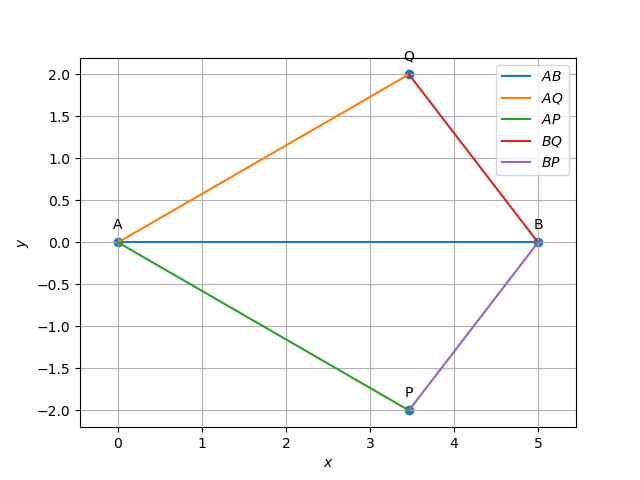
\includegraphics[width=\columnwidth]{fig_mat_comp.png}
    \caption{$\triangle APB \hspace{12pt} and \hspace{12pt} \triangle AQB$}
    %\label{fig:enter-label}
\end{figure}
\end{enumerate}
\end{enumerate}
%
\end{document} 
